\chapter{Evaluation}
%\note{This is where Assessors will be looking for signs of success and for evidence of thorough and systematic evaluation as discussed in Section 8.3. Sample output, tables of timings and photographs of workstation screens, oscilloscope traces or circuit boards may be included. A graph that does not indicate confidence intervals will generally leave a professional scientist with a negative impression.}

%\note{As with code, voluminous examples of sample output are usually best left to appendices or omitted altogether.}

%\note{There are some obvious questions which this chapter will address. How many of the original goals were achieved? Were they proved to have been achieved? Did the program, hardware, or theory really work?}

%\note{Assessors are well aware that large programs will very likely include some residual bugs. It should always be possible to demonstrate that a program works in simple cases and it is instructive to demonstrate how close it is to working in a really ambitious case.}

In my evaluation I explain the testing procedures I used to ensure that the compiler can correctly compile the OCaml subset, and compare the performance of my compiler with and without optimisations enabled to other compilers. In my proposal I stated that I would use Unit tests, with the possibility of an automated end to end tester depending on how complex it be to create. Thanks to NodeJS, I found that implementing an end to end tester was much simpler, and hence the end to end tester is the main system I used to both test my project and, with added benchmarking capabilities, evaluate it.
\\\\
In addition to using NodeJS I performed a manual check to ensure that both Chrome and Firefox could load WebAssembly modules compiled using the compiler.

\section{End To End Tester}
%\note{Could do with a -all mode to test all combinations of disabled / enabled optimisations. Or really just write a script to do that, will the examiners really be sitting there thinking `but did he test with every possible optimisation enable/disabled settings there could be'}

The end to end tester is the main method I have used to test the compiler. It can compile and execute a collection of 26 sample OCaml programs, testing their outputs against known correct values and running benchmarks against four benchmark samples --- comparing the performance of the WebAssembly against four other methods of executing the OCaml programs.
\\\\
It is a really useful tool because when new samples throw up problems with the compiler, they remain in the samples repository after the problem is fixed, thus acting as regression tests and preventing the same problem from occurring again undetected. As the end to end tester is quite fast to execute, it can be invoked after every code change to ensure that nothing has been broken, and it reduces the need for unit tests: as most bugs are detected by new code samples, there is no need to introduce a unit tests for the broken component because the end to end tester, having detected the bug, can attest to the bug not being there if the sample then compiles and tests correctly later.
\\\\
The End To End tester operates in several phases, each of which can detect problems: (Figure \ref{fig:sample} shows a sample and its corresponding JSON file)
\begin{enumerate}
	\item Compiling the OCaml program to WebAssembly Text Format using the compiler. If this compilation fails, an error is reported.
	\item Compiling WebAssembly Text Format to WebAssembly Binary Format using \textinline{wat2wasm}. This tool also verifies the WebAssembly programs, reporting issues such as a float value being stored into an integer variable.
	\item Loading and instantiating the WebAssembly program in Node.js. This runs the init function --- top-level code from the OCaml file which initializes global variables and can itself be arbitrarily complex. This could fail for instance if there is a problem executing this top-level code.
	\item Testing of global variable values against expected values. Most OCaml samples are accompanied by a JSON file which specifies these. For example, see figure \ref{fig:sample}.
	\item Execution of test functions: the JSON file can also specify functions with arguments and an expected result to execute, for instance \textinline{"gcd(15,25)": 5}.
	\item Execution of benchmarks: The JSON specifies a list of functions of type \camlinline{unit -> unit}, together with the number of iterations to perform on each function. These are then executed inside the WebAssembly environment and by compiling and executing for four other environments: the OCaml REPL interpreter, OCaml bytecode, optimised OCaml native code, and Js\_of\_OCaml.
\end{enumerate}
\begin{figure}[h]
	\begin{minipage}[t]{0.5\linewidth}
		\begin{minted}[linenos]{OCaml}
let sum x y = x + y

let ten = sum 8 2

let add4 = sum 4

let five = add4 1

let eight = add4 4
		\end{minted}
	\end{minipage}
	\begin{minipage}[t]{0.5\linewidth}
		\begin{minted}[linenos]{JSON}
{
  "globals": {
    "ten": 10,
    "five": 5,
    "eight": 8
  },
  "functions": {
    "sum(50,25)": 75
  }
}
		\end{minted}
	\end{minipage}
	\caption{\textinline{closure_basic.ml} sample and the corresponding JSON file}
	\label{fig:sample}
\end{figure}
In addition, command line arguments can be passed to the end to end tester to disable certain optimisations, which can be used both to test that the compiler still works with optimisations disabled, and to benchmark these optimisations.
\\\\
The samples cover all features that my compiler supports. Some samples are small, for testing that a particular feature works as intended such as the \textinline{tailrec.ml} sample which contains two tail-recursive functions: one with integer arguments and result, and the other with floating point arguments and result. Other samples are large and intend to show that lots of features can work together, for instance \textinline{core-subset.ml} intends to ensure that all features in the `core subset' that I defined as being the features I needed to support to meet the success criteria work.

\section{Benchmark Methodology}
%\note{
%	\begin{itemize}
%		\item Gcd: main target of optimisations. Went from 122ms to 8ms thanks to all of them.
%		\item others: they improve (e.g. especially with direct call generation), but not as much with the other optimisations
%		\item Make some performance graphs of the final result vs other execution engines, and of different optimisations enabled/disabled (can do both time and memory for that).
%	\end{itemize}
%}

Benchmarking allows the performance of my compiler to be compared with other methods of compiling and executing OCaml programs, and with various optimisations enabled and disabled. Most commonly, the execution time of samples is compared, with smaller values being beneficial as if code is executed faster, we can do more in a given period of time, and users spend less time waiting for computations. Memory usage is also important to benchmark, and reducing memory usage allows programs to run with larger input sizes on systems with constrained memory. Lastly, the size of programs can also be compared; smaller programs take less time to download, useful for WebAssembly applications which are always downloaded prior to execution (although some browsers may cache them).
\\\\
I benchmarked my compiler against four other execution environments: Three from the OCaml compiler toolchain and one alternative way of executing OCaml on the web. From the OCaml compiler I included the read-evaluate-print-loop (repl), executing compiled bytecode (byte) and compiled native code (nat). For executing OCaml on the web, I benchmarked against Js\_of\_OCaml (js) \cite{Js_of_ocaml}, a tool for converting OCaml bytecode into executable JavaScript.
\\\\
I selected four samples to be used as a benchmark:
\begin{itemize}
	\item GCD is a recursive implementation of greatest-common-divisor making use of a match statement
	\item Fibonacci is an implementation of the Fibonacci sequence using lazy-lists to repeatedly compute the 50th element
	\item Primes is an inefficient implementation of a lazy list of prime numbers featuring mutually recursive functions, repeatedly generating the 100th prime.
	\item Quicksort is a recursive implementation of Quicksort using lists.
\end{itemize}
I also chose different configurations of my compiler. (Abbreviations for my compiler are in capitals to distinguish them from the other execution environments):
\begin{itemize}
	\item AOE (All Optimisations Enabled) has all optimisations enabled
	\item NRE (No Ref Elimination) disables only reference elimination, since references only appear in tail-recursive functions after tail-recursion optimisation is performed
	\item NTC (No Tail Calls) additionally disables tail call optimisation.
	\item NIRO (No IR Optimisations) additionally disables the IR data-flow optimisations
	\item NDC (No direct calls) additionally disables direct call optimisation
	\item NSC (No stack codegen) additionally disables the stack code generator, using a linear algorithm instead.
\end{itemize}
Time benchmarks were performed for WebAssembly by using JavaScript to time in-between calls and returns from the WebAssembly function being benchmarked. For the other platforms, OCaml standard library code was injected into the benchmark code to time the benchmark function and output to standard output, however my compiler does not support compiling standard library functions, hence the JavaScript approach. The results of time benchmarks are shown in the top two plots of figures \ref{fig:timebenchgcdprime} and \ref{fig:timebenchfibquick}.
\\\\
Additionally, WebAssembly memory use was benchmarked, by comparing the \wainline{$mem_idx} global variable, indicating the address of the next free memory, before and after benchmarks were executed. Finally, by using the \textinline{wc} command line counts of the sample directory were also obtained. Memory results are shown at the bottom of figure \ref{fig:timebenchgcdprime} and code-length results are shown at the bottom of figure \ref{fig:timebenchfibquick}.

\begin{figure}[h]
	\begin{tikzpicture}
	\begin{axis}
	[
	width=\linewidth,
	height=0.55\linewidth,
	title=GCD Sample Benchmark Results,
	ylabel=Time (ms),
	boxplot/draw direction=y,
	xtick={1,2,3,4,5,6,7,8,9,10},
	xticklabels={repl, byte, js, nat, AOE, NRE, NTC, NIRO, NDC, NSC},
	minor y tick num=4,
	ymin=0,
	cycle list={{blue}, {red}, {teal}, {black}},
	]
	\addplot+[ boxplot prepared={lower whisker=46.916799999999995, lower quartile=46.9739690495893, median=47.54592600000001, upper quartile=48.11788295041072, upper whisker=50.520999999999994  }, ] coordinates {};
	\addplot+[ boxplot prepared={lower whisker=39.3934, lower quartile=39.629678719549936, median=40.625997999999996, upper quartile=41.622317280450055, upper whisker=43.497  }, ] coordinates {};
	\addplot+[ boxplot prepared={lower whisker=2.79998779297, lower quartile=2.79998779297, median=2.9419999122631992, upper quartile=3.3774727283827337, upper whisker=5.299997329710001  }, ] coordinates {};
	\addplot+[ boxplot prepared={lower whisker=2.0927, lower quartile=2.0927, median=2.6599920000000004, upper quartile=3.5743190467048436, upper whisker=5.004700000000001  }, ] coordinates {};
	\addplot+[ boxplot prepared={lower whisker=1.9, lower quartile=1.9, median=2.4459999999999997, upper quartile=3.2319287499512948, upper whisker=3.8  }, ] coordinates {};
	\addplot+[ boxplot prepared={lower whisker=6.4, lower quartile=6.453060024019196, median=6.528, upper quartile=6.602939975980803, upper whisker=6.7  }, ] coordinates {};
	\addplot+[ boxplot prepared={lower whisker=14.1, lower quartile=14.1, median=14.164000000000009, upper quartile=14.240837490847637, upper whisker=14.4  }, ] coordinates {};
	\addplot+[ boxplot prepared={lower whisker=26.2, lower quartile=26.2, median=26.657999999999987, upper quartile=28.4975749509059, upper whisker=39.5  }, ] coordinates {};
	\addplot+[ boxplot prepared={lower whisker=87, lower quartile=87, median=88.03, upper quartile=91.97703686326844, upper whisker=115.5  }, ] coordinates {};
	\addplot+[ boxplot prepared={lower whisker=85.5, lower quartile=85.5, median=86.38, upper quartile=90.03316301306162, upper whisker=111.5  }, ] coordinates {};
	\end{axis}
	\end{tikzpicture}
	\begin{tikzpicture}
	\begin{axis}
	[
	width=\linewidth,
	height=0.55\linewidth,
	title=Primes Sample Benchmark Results,
	ylabel=Time (ms),
	boxplot/draw direction=y,
	xtick={1,2,3,4,5,6,7,8,9,10},
	xticklabels={repl, byte, js, nat, AOE, NRE, NTC, NIRO, NDC, NSC},
	minor y tick num=4,
	ymin=0,
	cycle list={{blue}, {red}, {teal}, {black}},
	]
	\addplot+[ boxplot prepared={lower whisker=440.0005, lower quartile=443.729268814417, median=453.1682800000001, upper quartile=462.60729118558316, upper whisker=475.711  }, ] coordinates {};
	\addplot+[ boxplot prepared={lower whisker=453.51750000000004, lower quartile=460.86905941993587, median=475.08469, upper quartile=489.3003205800642, upper whisker=518.2655000000001  }, ] coordinates {};
	\addplot+[ boxplot prepared={lower whisker=565.9999847400001, lower quartile=578.9949765768573, median=604.2200040816, upper quartile=629.4450315863427, upper whisker=663.4999513649999  }, ] coordinates {};
	\addplot+[ boxplot prepared={lower whisker=136.5105, lower quartile=136.6669762870124, median=144.18178999999998, upper quartile=151.69660371298755, upper whisker=167.15650000000002  }, ] coordinates {};
	\addplot+[ boxplot prepared={lower whisker=407, lower quartile=407, median=419.89, upper quartile=437.9297588675684, upper whisker=531  }, ] coordinates {};
	\addplot+[ boxplot prepared={lower whisker=482.5, lower quartile=482.5, median=487.88, upper quartile=514.2042397800961, upper whisker=672  }, ] coordinates {};
	\addplot+[ boxplot prepared={lower whisker=354, lower quartile=354, median=358.91, upper quartile=378.8871594577406, upper whisker=497  }, ] coordinates {};
	\addplot+[ boxplot prepared={lower whisker=354, lower quartile=354, median=358.49, upper quartile=378.5843997173342, upper whisker=498.5  }, ] coordinates {};
	\addplot+[ boxplot prepared={lower whisker=529, lower quartile=529, median=537, upper quartile=561.4989795705865, upper whisker=703  }, ] coordinates {};
	\addplot+[ boxplot prepared={lower whisker=533, lower quartile=533, median=540.28, upper quartile=563.855444852644, upper whisker=702  }, ] coordinates {};
	\end{axis}
	\end{tikzpicture}
	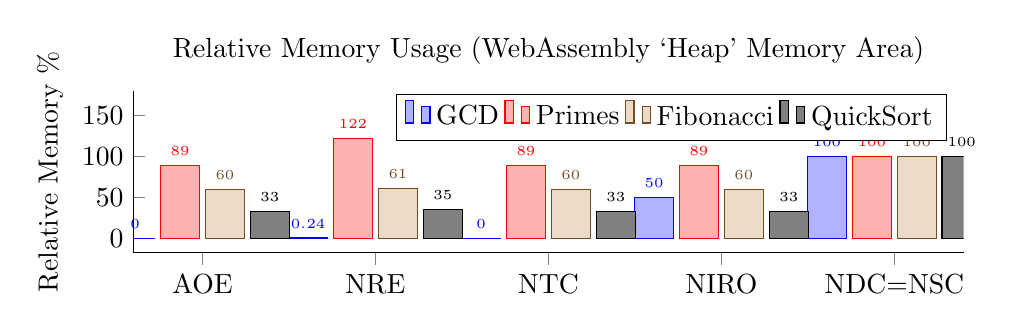
\begin{tikzpicture}
\begin{axis}
[
width=\linewidth,
height=0.3\linewidth,
title=Relative Memory Usage (WebAssembly `Heap' Memory Area),
ylabel=Relative Memory \%,
xtick={1,2,3,4,5},
xticklabels={AOE, NRE, NTC, NIRO, NDC=NSC},
nodes near coords,
every node near coord/.append style={font=\tiny},
ybar,
ymax=180,
axis x line*=bottom,
axis y line*=left,
bar width = 0.5cm,
legend columns=4
]
%	\addplot coordinates {(1, 0) (2,0.012) (3, 0) (4, 2.49) (5, 4.97)};
%	\addplot coordinates {(1,314) (2,432) (3,314) (4,314) (5,356)};
%	\addplot coordinates {(1,11.9) (2,12.0) (3,11.9) (4,11.9) (5,19.9)};
%	\addplot coordinates {(1,26.9) (2,29.0) (3,26.9) (4,26.9) (5,82.3)};

\addplot coordinates {(1,0) (2,0.24) (3,0) (4,50) (5,100)};
\addplot coordinates {(1,89) (2,122) (3,89) (4,89) (5,100)};
\addplot coordinates {(1,60) (2,61) (3,60) (4,60) (5,100)};
\addplot coordinates {(1,33) (2,35) (3,33) (4,33) (5,100)};
\legend{GCD, Primes, Fibonacci, QuickSort}

\end{axis}
\end{tikzpicture}
	\caption{Time Benchmark Results for GCD and Primes, and Memory Benchmark Results}
	\label{fig:timebenchgcdprime}
\end{figure}
\begin{figure}[h]
	\begin{tikzpicture}
	\begin{axis}
	[
	width=\linewidth,
	height=0.55\linewidth,
	title=Fibonacci Sample Benchmark Results,
	ylabel=Time (ms),
	boxplot/draw direction=y,
	xtick={1,2,3,4,5,6,7,8,9,10},
	xticklabels={repl, byte, js, nat, AOE, NRE, NTC, NIRO, NDC, NSC},
	minor y tick num=4,
	ymin=0,
	cycle list={{blue}, {red}, {teal}, {black}},
	]
	\addplot+[ boxplot prepared={lower whisker=15.467199999999997, lower quartile=15.608607416911102, median=16.368972, upper quartile=17.129336583088897, upper whisker=20.128800000000002  }, ] coordinates {};
	\addplot+[ boxplot prepared={lower whisker=14.551600000000002, lower quartile=14.551600000000002, median=15.991112000000001, upper quartile=17.765839039365794, upper whisker=22.833000000000002  }, ] coordinates {};
	\addplot+[ boxplot prepared={lower whisker=24.399995803800003, lower quartile=25.483233126240698, median=27.460002899176, upper quartile=29.436772672111303, upper whisker=34.4000339508  }, ] coordinates {};
	\addplot+[ boxplot prepared={lower whisker=2.3004000000000002, lower quartile=2.6957899532811833, median=3.608784, upper quartile=4.521778046718817, upper whisker=4.6146  }, ] coordinates {};
	\addplot+[ boxplot prepared={lower whisker=11.8, lower quartile=12.43774826419513, median=13.86, upper quartile=15.282251735804868, upper whisker=18.8  }, ] coordinates {};
	\addplot+[ boxplot prepared={lower whisker=11, lower quartile=11, median=11.403999999999998, upper quartile=12.252989988162408, upper whisker=17  }, ] coordinates {};
	\addplot+[ boxplot prepared={lower whisker=10.6, lower quartile=10.6, median=11.036000000000003, upper quartile=11.915718136677851, upper whisker=17  }, ] coordinates {};
	\addplot+[ boxplot prepared={lower whisker=10.8, lower quartile=10.8, median=11.204000000000002, upper quartile=12.10065154881925, upper whisker=17.2  }, ] coordinates {};
	\addplot+[ boxplot prepared={lower whisker=29, lower quartile=29, median=29.89, upper quartile=31.53708834007165, upper whisker=40.5  }, ] coordinates {};
	\addplot+[ boxplot prepared={lower whisker=30, lower quartile=30, median=30.92, upper quartile=32.22904545375626, upper whisker=37  }, ] coordinates {};
	\end{axis}
	\end{tikzpicture}
	\begin{tikzpicture}
	\begin{axis}
	[
	width=\linewidth,
	height=0.55\linewidth,
	title=Quicksort Sample Benchmark Results,
	ylabel=Time (ms),
	boxplot/draw direction=y,
	xtick={1,2,3,4,5,6,7,8,9,10},
	xticklabels={repl, byte, js, nat, AOE, NRE, NTC, NIRO, NDC, NSC},
	minor y tick num=4,
	ymin=0,
	cycle list={{blue}, {red}, {teal}, {black}},
	]
	\addplot+[ boxplot prepared={lower whisker=56.8678, lower quartile=56.91425603242595, median=57.98698800000001, upper quartile=59.05971996757407, upper whisker=61.493599999999994  }, ] coordinates {};
	\addplot+[ boxplot prepared={lower whisker=55.09159999999999, lower quartile=55.52400983224097, median=58.515055999999994, upper quartile=61.50610216775902, upper whisker=66.2124  }, ] coordinates {};
	\addplot+[ boxplot prepared={lower whisker=47.399997711199994, lower quartile=47.85241953213496, median=50.64800262451201, upper quartile=53.44358571688906, upper whisker=58.399963379  }, ] coordinates {};
	\addplot+[ boxplot prepared={lower whisker=19.3928, lower quartile=19.423863834523758, median=23.019788000000002, upper quartile=26.615712165476246, upper whisker=33.4728  }, ] coordinates {};
	\addplot+[ boxplot prepared={lower whisker=28.2, lower quartile=28.289955717442474, median=31.31600000000001, upper quartile=34.342044282557545, upper whisker=39  }, ] coordinates {};
	\addplot+[ boxplot prepared={lower whisker=25.6, lower quartile=25.6, median=26.55199999999999, upper quartile=28.56418687004973, upper whisker=40.4  }, ] coordinates {};
	\addplot+[ boxplot prepared={lower whisker=26, lower quartile=26, median=26.667999999999996, upper quartile=28.60153975909475, upper whisker=40  }, ] coordinates {};
	\addplot+[ boxplot prepared={lower whisker=26, lower quartile=26, median=26.992000000000008, upper quartile=28.83415525947174, upper whisker=39.6  }, ] coordinates {};
	\addplot+[ boxplot prepared={lower whisker=97, lower quartile=97, median=99.54, upper quartile=105.46523417258754, upper whisker=140  }, ] coordinates {};
	\addplot+[ boxplot prepared={lower whisker=99, lower quartile=99, median=102.04, upper quartile=108.64896361012822, upper whisker=147  }, ] coordinates {};
	\end{axis}
	\end{tikzpicture}
	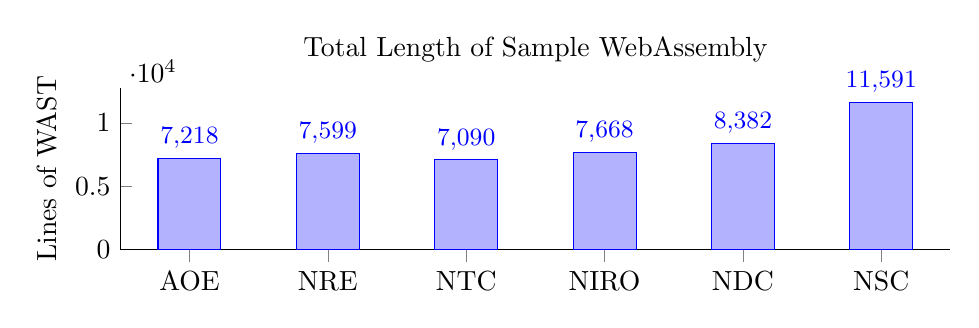
\begin{tikzpicture}
\begin{axis}
[
width=\linewidth,
height=0.3\linewidth,
title=Total Length of Sample WebAssembly,
ylabel=Lines of WAST,
xtick={1,2,3,4,5,6},
xticklabels={AOE, NRE, NTC, NIRO, NDC, NSC},
nodes near coords,
every node near coord/.append style={font=\small},
ymin=0,
ybar,
axis x line*=bottom,
axis y line*=left,
bar width = 0.8cm,
]
%	\addplot coordinates {(1, 0) (2,0.012) (3, 0) (4, 2.49) (5, 4.97)};
%	\addplot coordinates {(1,314) (2,432) (3,314) (4,314) (5,356)};
%	\addplot coordinates {(1,11.9) (2,12.0) (3,11.9) (4,11.9) (5,19.9)};
%	\addplot coordinates {(1,26.9) (2,29.0) (3,26.9) (4,26.9) (5,82.3)};

\addplot coordinates {(1,7218) (2,7599) (3,7090) (4,7668) (5,8382) (6, 11591)};

\end{axis}
\end{tikzpicture}
	\caption{Time Benchmark Results for GCD and Primes, and Code Length Benchmark Results}
	\label{fig:timebenchfibquick}
\end{figure}

\section{Benchmark Results}
The results are promising: my compiler's WebAssembly is executed faster than the OCaml bytecode and Js\_of\_OCaml for all four benchmarks, and is hence a viable method for executing OCaml code on the web. There are however significant drawbacks: my code does not have to expend time performing garbage collection, and the lack of garbage collection means it is unlikely to be a good choice for executing high-memory-usage OCaml programs. Additionally, OCaml developers in practice use a standard library and split their code across multiple files, both features unsupported by my compiler and hence making it a more difficult to use tool for compiling OCaml for the web.
\\\\
Overall, the optimisations lead to significant speed-ups on all samples, with GCD's average execution time going from 86.4ms to 2.4ms, a reduction of 97\%. Primes' average execution time was reduced from 540.3ms to 419.9ms (22\% improvement), however with tail-call optimisation disabled this improves to 358.9ms (34\% improvement). There are many interesting observations to be made from the results for various optimisations:

\subsubsection{Stack Code Generation}
This optimisation clearly shows a significant line-of-code reduction of 3209 lines across all samples, although without a notable improvement in execution time. This is likely due to additional optimisations and compilation that WebAssembly goes under before it is executed: it must be compiled to register-based machine code, in practice removing the difference between accessing values on the stack and values stored in WebAssembly variables, both of which will likely become register accesses. In the case of GCD, we see execution time is slightly worsened with this optimisation, potentially a by-product of the stack code generator's ability to store a value on the stack for a long time until it is needed instead of storing it in a variable.

\subsubsection{Direct Calls}
Enabling this leads to a drastic improvement in execution time in all cases. GCD for instance executes in 26.5ms as opposed to 88ms. Memory usage also sees a great improvement due to the reduced need to construct closures as partial applications are replaced with full applications where possible. Finally, we also see a slight improvement in line-count, due to some memory operations for constructing closures being eliminated.

\subsubsection{IR Optimisations}
These only really effect the GCD sample, where dead-code elimination combined with tuple-load elimination leads to tuple-creation for the match statement being eliminated, thus reducing execution time and completely eliminating GCD's heap memory usage. In the other samples, optimisations alias-elimination can remove some variables and thus we see a reduction in the lines-of-code, but no improvement in execution time likely due to the WebAssembly environment's own optimisations when the WebAssembly is compiled to machine code.

\subsubsection{Tail Call Optimisation and Ref Elimination}
Enabling this optimisation cuts in half GCD's execution time compared to with just the previously discussed optimisations. However, for the other samples the result is either no improvement or an increase in execution time! A possible explanation for this is that GCD calls a tail-recursive function once that then loops many times, while other samples make many calls to tail-recursive functions that may loop only a few times, thus incurring the overhead of the loop and the `references' (eliminated with ref-elimination) without the gain if the loop is only used a few times. Primes for instance has mutually recursive functions that are tail-call optimised, but make frequent calls to each other.
\\\\
The increase in memory is due to the references, and is hence eliminated by ref-elimination. Lines-of-code also increases due to the additional loop code added to functions.

% TODO DONT FORGET ALL THE WORK IN MAKING THE CODE SHORTER

% TODO HOW IT WAS EVALUATED
% TODO TEST SYSTEM AND BENCHMARKS

